%---------------------------------------------------------------------------------------------------
% Aufgaben
%---------------------------------------------------------------------------------------------------
\newpage
%\part{Anfang}
\chapter{Aufgaben}
Aufgrund der in der Einarbeitung erworbenen Kenntnisse war es m\"oglich an folgenden Projekten zu partizipieren. Im Fokus stand die H2-Mobility App, mit einer geringeren Priorit\"at folgte die LFI App und zum Schluss gab es noch ein Projekt in dem eine sogenannte Launcher App entwickelt werden sollte. 

\section{Theorie}
Die vielf\"altigen  M\"oglichkeiten und Eigenschaften die Android Studio bietet k\"onnen im Rahmen dieses Praktikumsberichts nicht im Detail beschrieben werden. Daher wird hier nur auf die f\"ur die Aufgabenbew\"altigung wesentlichen Aspekte eingegangen. Dazu z\"ahlen besonders \textit{Activities} und \textit{Fragments}. Im folgenden wird dazu ein kurzer \"Uberblick pr\"asentiert und auschlie\ss{}end auf die verschiedenen Apps eingegangen.

\subsection{Activity}
Eine \textit{Activity} dient als Fenster in dem User Interface Elemente (UI) platziert sind, um mit dem Benutzer zu interagieren. Sie f�llt beinahe den gesamten Bildschirm des Ger�tes aus und implementiert verschiedene Methoden die dem Lifecycle der \textit{Activity} dienen und um die \textit{Activity} mit der zugeh�rigen .xml Datei zu verbinden. 

\subsection{Fragment}
\textit{Fragments} sind ein Teil der UI von der App und k�nnen in einer \textit{Activity} platziert werden. Sie geh\"oren demnach zu einer \textit{Activity}. Es ist auch m�glich mehrere \textit{Fragments} in einer \textit{Activity} zu platzieren. Der aktuell beste Ansatz ist es eine \textit{Activity} zu haben und den Rest �ber \textit{Fragments} zu realisieren. Abbildung (\ref{fig:lifecycleOverview}) zeigt eine \"Ubersicht zum \textit{Lifecycle} von \textit{Fragment} und \textit{Activity}.
%https://stackoverflow.com/questions/20306091/dilemma-when-to-use-fragments-vs-activities

\begin{figure}[H]
	\centering 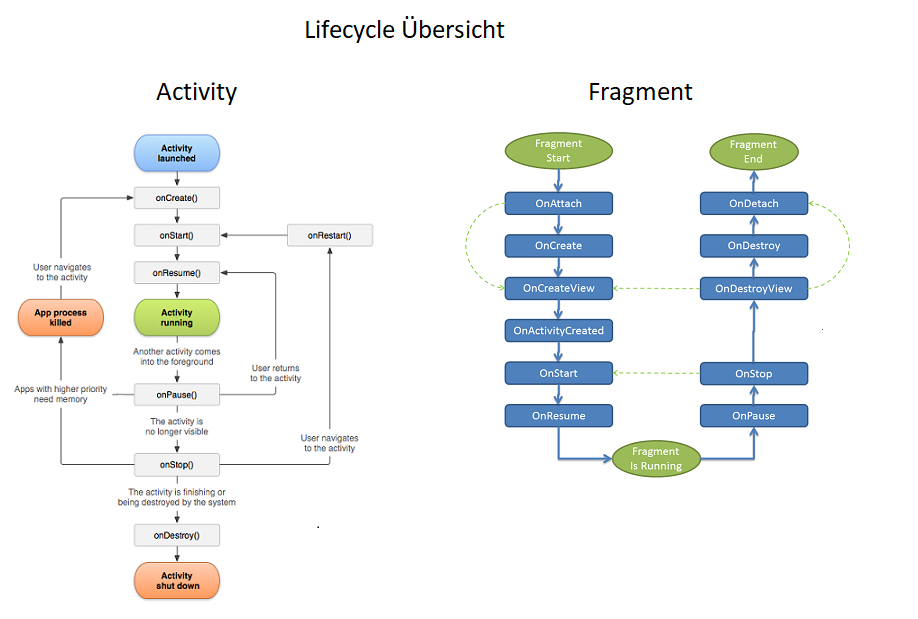
\includegraphics[width=0.8\textwidth]{lifecycleOverview.png}
	\caption[lifecycleOverview]{Prototyp der InVision Vorgabe. Feedback Button f\"ur konkret ausgew\"ahlte Tankstelle}
	\label{fig:lifecycleOverview}
\end{figure}
%https://developer.android.com/reference/android/app/Activity#ActivityLifecycle
%https://docs.microsoft.com/de-de/xamarin/android/platform/fragments/creating-a-fragment

% ----------------------------
\section{H2 Mobility App}
Die App ist f\"ur Besitzer von Wasserstoffautos, also Autos mit einer Brennstoffzelle, gedacht. "Die Brennstoffzelle wird sich durchsetzen"\footnotemark \footnotetext{URL: http://www.spiegel.de/auto/aktuell/wasserstoffauto-die-brennstoffzelle-wird-sich-durchsetzen-a-1235431.html}, ist sich Toyota-Motorenentwickler Gerald Killmann sicher. Daher hat die H2 Mobility Deutschland GmbH \& Co.KG die Firma portrix.net mit der Entwicklung einer App beauftragt die den Nutzern unter anderem das europ\"aische Tankstellennetz und die Route zur n\"achstgelegenen Tankstelle anzeigt, ein Feedback f\"ur die Tankstellenbetreiber, Schulungsvideos zum Tankvorgang und viele weitere Funktionen bietet. Zuk\"unftig soll es auch m\"oglich sein mittels Mobiltelefon samt App am Tankterminal zu bezahlen.
Die Entwicklung der App erfolgt nach R\"ucksprache mit dem Vertreter von H2 Mobility und dem f\"ur das Layout verantwortlichen Designer und wird sowohl f\"ur iOS als auch f\"ur Android bei portrix.net programmiert. Features und design-Prototypen werden \"uber das digitale Produkt Design Tool InVision an die Programmierer vermittelt und anschlie\ss{}end umgesetzt. Aufgrund der hohen Komplexit\"at und des Umfangs den die App mittlerweile angenommen hat, hat sich das Erscheinungsbild zwischenzeitlich stark ver\"andert. Das organische anwachsen der Funktionalit\"at ist am Versionskontrollbaum gut zu erkennen, da das Projekt beinahe 20000 commits enth\"alt.

\subsection{Feedback}
\"Uber InVision kam die Vorgabe einen Prototyp zu entwickeln, der es erm\"oglicht einer konkret ausgew\"ahlten Tankstelle per \textit{Button} ein Feedback zu geben.

\begin{figure}[H]
	\centering 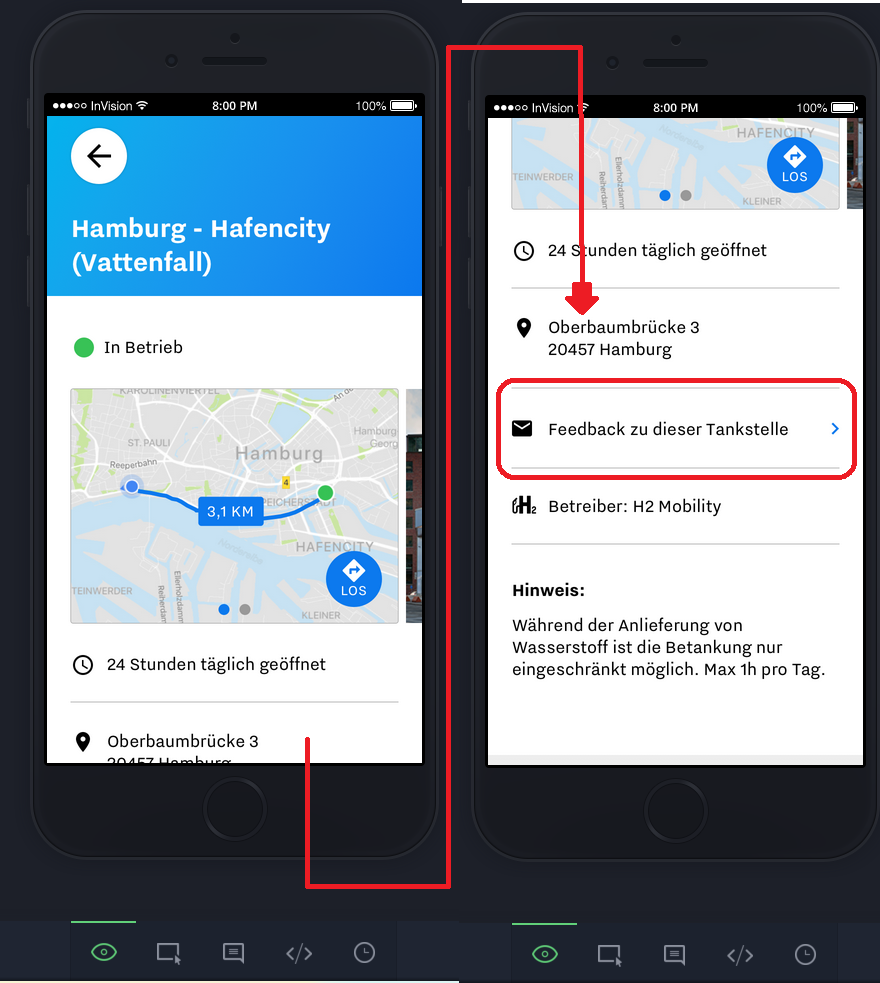
\includegraphics[width=0.8\textwidth]{feedbackPrototyp.png}
	\caption[FeedbackPrototyp]{Prototyp der InVision Vorgabe. Feedback Button f\"ur konkret ausgew\"ahlte Tankstelle}
	\label{fig:FeedbackPrototyp}
\end{figure}
%\footnotetext{URL: https://www.guitarchalk.com/wp-content/uploads/2017/07/electric-guitar-parts.jpg [cited 22 August 2018]}


In der bisherigen Version war es m\"oglich \"uber eine \textit{Button} in der FuelStationsMap.java (MainActivity) das HelpAndFeedback.java (\textit{Fragment}) aufzurufen und von dort in ein allgemeine Feedback.java (\textit{Fragment}) zu kommen Abb.(\ref{fig:inVisionFeedbackPrototyp}) (1 -> 2b -> 3). Dort l\"asst sich aus einem \textit{Spinner}, der jede Tankstelle auflistet, eine Tankstelle ausw\"ahlen. Es war also naheliegend den Code zu modifizieren, um aus der FuelStationDetail.java (\textit{Activity}) direkt in das Feedback.java zu wechseln und die angew\"ahlte Tankstelle direkt im Spinnerfeld anzuzeigen.
Hierzu mussten diverse \"Anderungen vorgenommen werden, da das Feedback.java der darunterliegenden FuelStationsMap.java geh\"ort und in der \textit{OnCreate()} Methode des Feedback.java eine FuelStationsMap Variable als \textit{Context} initialisiert wird (\ref{code:onCreate}). Dieser \textit{Context} gew\"ahrleistet unter anderem das der \textit{Spinner} im Feedback.java mit Daten der Tankstellen gef\"ullt werden kann. Der \textit{Context} macht es allerdings unm\"oglich das Feedback.java von einer weiteren \textit{Activity}, also der FuelStationDetail.java gestartet wird. Es war daher notwendig die FuelStationDetail.java (\textit{Activity}) als \textit{Fragment} nachzubauen. 
Der gew\"unschte workflow wird in Abb.(\ref{fig:inVisionFeedbackPrototyp}) dargestellt.

\begin{figure}[H]
	\centering 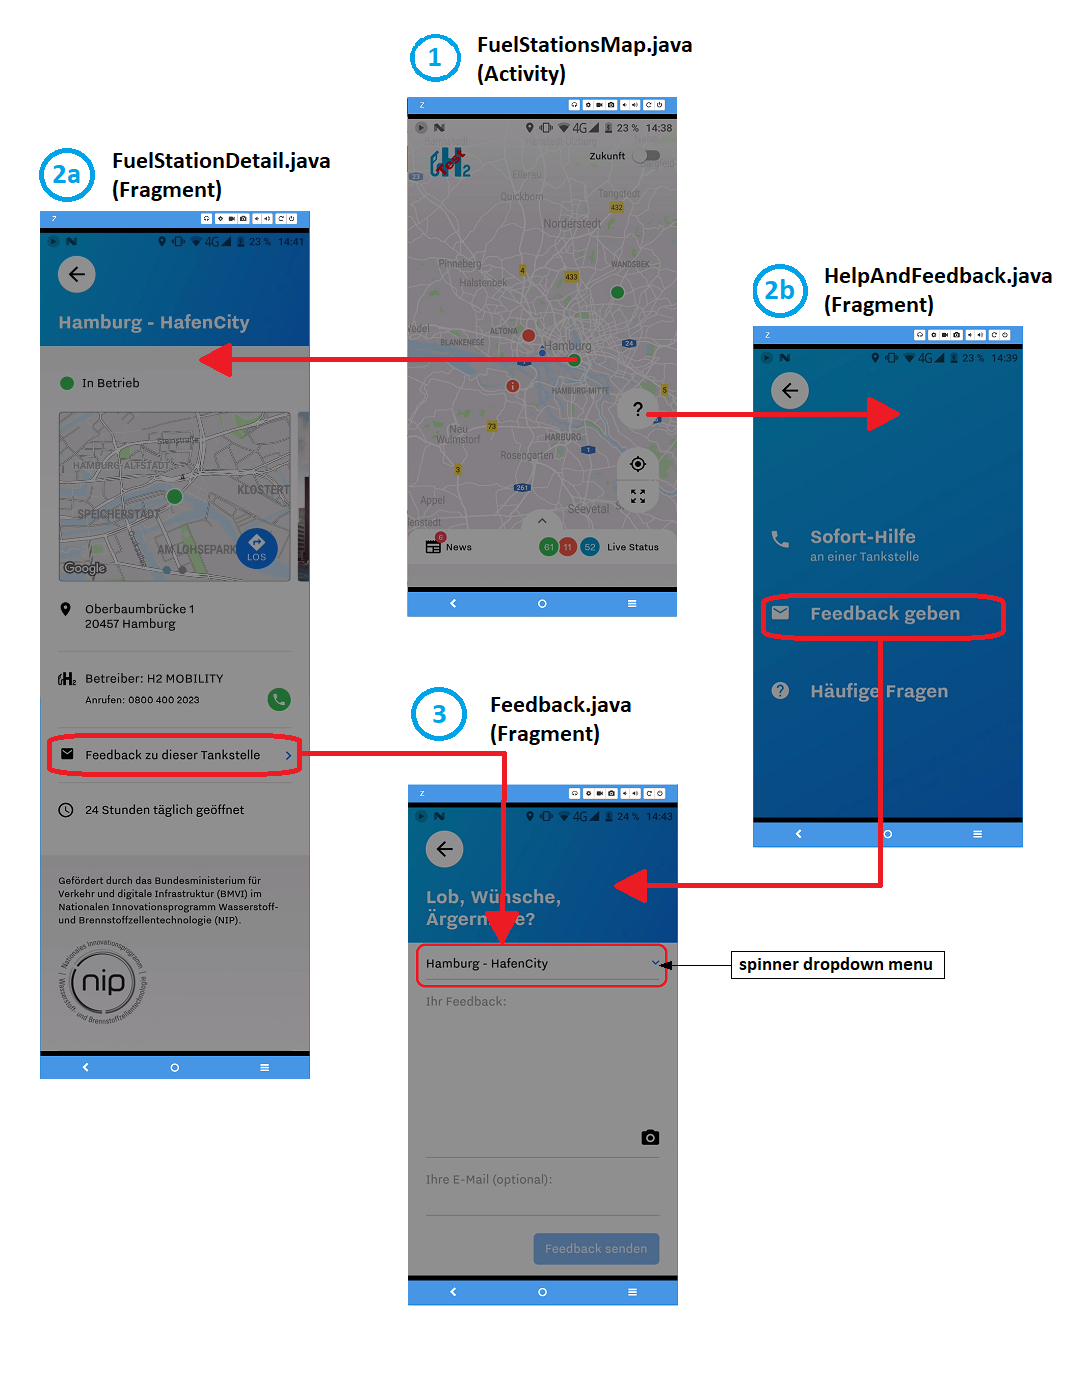
\includegraphics[width=0.8\textwidth]{inVisionFeedbackPrototyp.png}
	\caption[inVisionFeedbackPrototyp]{Workflow der neuen Feedback Funktion}
	\label{fig:inVisionFeedbackPrototyp}
\end{figure}


\fbox{
\lstinputlisting[label={code:onCreate} ,caption={onCreate() Methode der Feedback.java},captionpos=b, language = java,  numbers = left]{program/Feedback.java}
}

Das Layout einer App wird in der zur \textit{Activity} bzw. \textit{Fragment} zugeh\"origen .xml Datei definiert. In diesem Fall konnte der meiste Inhalt aus der activity\_fuel\_station\_detail.xml in die neue fragment\_fuel\_station\_detail.xml kopiert und um das gew\"unschte neue Feature erg\"anzt werden (\ref{code:feedbackXml}). 


\fbox{
\lstinputlisting[label={code:feedbackXml} ,caption={Designelement Feedback Button},captionpos=b, language = xml,  numbers = left]{program/fragment_fuel_station_detail.xml}
}

Der Transfer (1 -> 2a) erfolgt durch anklicken eines Tankstellen \textit{Markers}. Die bisherige Logik rief die FuelStationDetail.java (\textit{Activity}) auf und musste durch eine \textit{Fragment Transaction} ersetzt werden. Zu sehen in Abb.(\ref{code:markerTransaction})
Beim Aufruf von \textit{onMarkerClick()} wird der angeklickte \textit{Marker} als Argument �bergeben. Es wird �ber die MapHelper Klasse eine FuelStation Variable station zugewiesen und dessen idx, wenn die station ungleich null ist in ein \textit{Bundle} gespeichert. Dieses \textit{Bundle} b wird einem neuen FuelStationDetail (\textit{Fragment}) als Argument �bergeben und anschlie\ss{}end wird mit dem \textit{SupportFragmentManager} die \textit{Fragment Transaction} zum FuelStationDetail mit ausgew�hlter FuelStation.

\fbox{
\lstinputlisting[label={code:markerTransaction} ,caption={Wechsel von FuelStationsMap zu FuelStationDetail},captionpos=b, language = java,  numbers = left]{program/MarkerTransaction.java}
}


Um �ber die Detailansicht der Tankstelle zum gew�nschten Feedback (2a -> 3) zu gelangen muss die ID des FrameLayout lyFeedbackPin deklariert und initialisiert werden und anschlie\ss{}end \"uber einen onClickListener() angeklickt werden. Siehe Abb.(\ref{code:transaction}). Das Prozedere ist dem vorangegangenem \"ahnlich. Der unterschied besteht darin das in der onClick() Methode das Bundle b �ber getArguments() den Marker �bergeben bekommt und an das Feedback.java weiterreicht, damit dort das Spinner field menu den Tankstellen namen vorausw�hlen kann. Die eigentliche Transaktion von FuelStationDetail zu Feedback funktioniert nach dem gleichen Muster wie zuvor beschrieben.

\fbox{
\lstinputlisting[label={code:transaction} ,caption={Wechsel von FuelStationDetail zu Feedback},captionpos=bl, language = java,  numbers = left]{program/Transaction.java}
}

%--------------
%design vorgabe von Invision
%direktes Feedback im Fragment
%-----------
\subsection{Opt-Out}
Um das Nutzerverhalten der App zu verbessern werden s\"amtliche Interaktionen des Benutzers mithilfe von \textit{Google Analytics} registriert. Aufgrund der Datenschutzgrundverordnung\footnotemark \footnotetext{URL: https://www.121watt.de/online-marketing/google-analytics-datenschutz-konform/} (DSVGO) muss es dem Benutzer m�glich sein dies zu deaktivieren. Dazu bietet Google Analytics die sogenannte Opt-Out Funktion an. Der "Google Analytics deaktivieren"  \textit{Button} befindet sich im Impressum (Abb.(\ref{fig:impressum})). Das Impressum ist ein \textit{WebView} indem die Url des Impressums der H2.Live Webseite aufgerufen und angezeigt wird. Die HTML (\ref{fig:impressum}) enth�lt JavaScript Elemente die in der App ausgelesen und interpretiert werden, wenn der \textit{Button} gedr�ckt wird.  

\begin{figure}[H]
	\centering 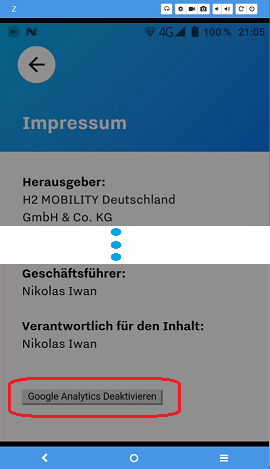
\includegraphics[width=0.4\textwidth]{impressum.png}
	\caption[impressum]{Impressum mit Google Analytics deaktivieren Button}
	\label{fig:impressum}
\end{figure}

Abbildung (\ref{code:optout}) (Zeile 7) zeigt das Html Code\-Segment in dem der "Google Analytics Deaktivieren" Button definiert wird und ab Zeile 13 wird mit JavaScript beschrieben, was f�r die verschiedenen Betriebssysteme bei Knopfdruck passieren soll. Zeile 20 beschreibt das verhalten f�r Android und Zeile 22 f�r iOS. Es ist von entscheidender Bedeutung, dass die Klassen, Methoden und Objekte im Java\-Code die gleichen Namen haben wie im JavaScript. Damit der Java\-Code JavaScript interpretieren kann muss ein JavaScript\-Interface implementiert werden. In Abbildung (\ref{code:webview} ist zu sehen, wie in der inneren Java Klasse GoogleAnalytics.java die Methode postMessage() aufgerufen und als Argument ein JsonObject mit dem Property "action" �bergeben wird. Wenn dieses "action" Property "optOut" als Wert beinhaltet wird der Google Analytics Tracker deaktiviert indem der Methode setTrackerOptOut(true) als Argument �bergeben wird. Die Implementierung des JavaScript\-Interface erfolgt durch die "@"\-Annotation in Zeile 1 und schlie\ss{}lich durch das verbinden der Java Klasse "GoogleAnalytics()" mit der JavaScript Klasse "googleAnalytics" (Zeile 22).

\fbox{
\lstinputlisting[label={code:optout} ,caption={Html des Impressums},captionpos=b, language = html,  numbers = left]{program/optout.html}
}

\fbox{
\lstinputlisting[label={code:webview},caption={Interpretation von JavaScript in Android Studio},captionpos=b, language = html,  numbers = left]{program/webview.java}
}


% ----------------------------
\section{LFI App}
super fotografie app
\subsection{Magazin Overview}
neugestaltung der Magazin ansicht
\subsection{Magazin Preview}
Magazin vorschau mit 10 beispielseiten

% ----------------------------
\section{Launcher App}
angesagte Spiegel Tablet